\q{5}{One, two, three}

\begin{enumerate}
\item How many ways can we roll 3 dice, such that they are in a strictly decreasing sequence? 


% \solution{
% This would simply be $\binom{6}{3}$, because given any combination there is exactly 1 strictly decreasing sequence (and we can get all the strictly decreasing sequences). 
% }
\vspace{5cm}

\item How many rectangles are in the following grid? 
\begin{center}
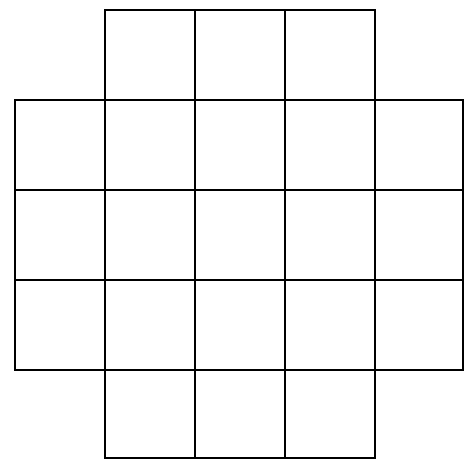
\includegraphics{grid.png}
\end{center}
\

% \solution{
% We count the number of rectangles in the 5 x 5 grid, then subtract each of the cases. We have $\binom{6}{2} ^2 - 4^3 - 4^2 - 0 - 1 = \square{144}$. 
% }
\end{enumerate}
